\subsection{PD-Regler} % (fold)
\label{sub:PD-Regler}
\begin{frame}
    \frametitle{PD-Regler}
    \framesubtitle{}
    \begin{block}{Versuch}
        \begin{itemize}
            \item Zusammenspiel von P und D
        \end{itemize}    
    \end{block}
\end{frame}
\begin{frame}
    \frametitle{Messung}
    \framesubtitle{}
     \begin{columns}[c]
        \column{0.6\textwidth}
        \begin{alertblock}{Problem}
             \begin{itemize}
                 \item Sehr starke Störungen
                 \item Gründe
                 \begin{itemize}
                     \item Platz an der Tür
                     \item Klimaanlage
                 \end{itemize}
                 \item T pendelt sich nicht wirklich ein
                 \item keine aufschlussreichen Messungen möglich
             \end{itemize}
        \end{alertblock}
        \begin{block}{Messung}
            \begin{itemize}
                \item ungedämpfte Schwungung ab ca. $k_p=4.6$
                \item D-Regler dämpft Schwingung ab
            \end{itemize}
        \end{block}
        \column{0.4\textwidth}
        \begin{figure}[H]
        \begin{center}
                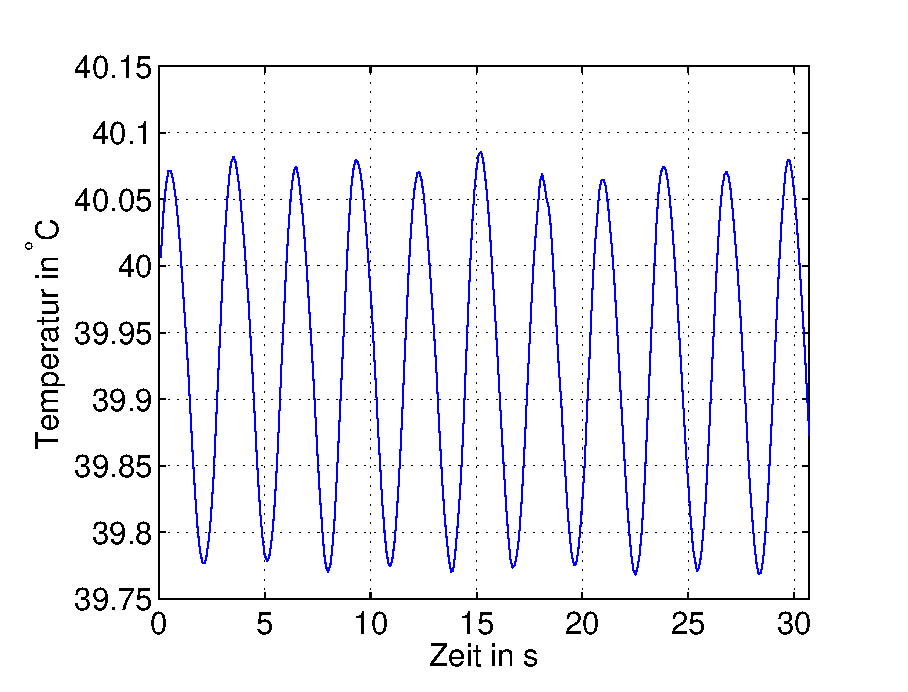
\includegraphics[scale=0.3]{./img/plots/2f_4_6.eps}
        \end{center}
        \end{figure}
        \begin{figure}[H]
        \begin{center}
                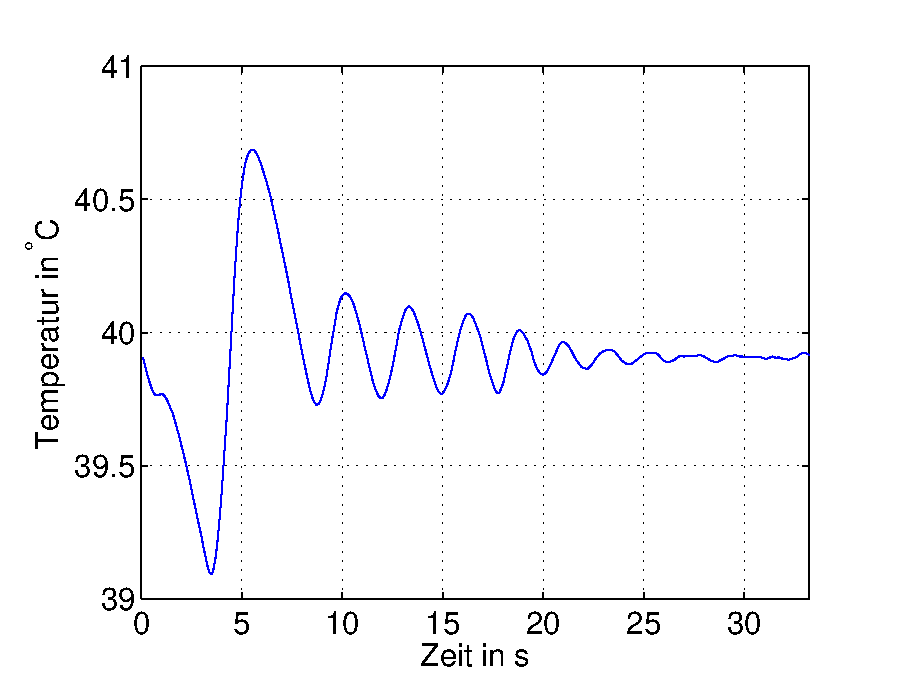
\includegraphics[scale=0.2]{./img/plots/2f_4_6_td1.eps}
        \end{center}
        \end{figure}
     \end{columns}
\end{frame}

% subsection PD-Regler (end)
